\documentclass[twoside,12pt]{mythesis} %this is the mythesis.cls file
% twoside,openright,versioninfo

% Consider:
% \newcommand{\ie}{i.\,e.}
% \newcommand{\Ie}{I.\,e.}
% \newcommand{\eg}{e.\,g.}
% \newcommand{\Eg}{E.\,g.}
\usepackage{graphicx}
\usepackage{amsmath}
\usepackage{booktabs}
\usepackage{pdfpages} % new addition
\usepackage{xparse}
\usepackage{float}
\usepackage{setspace} % new addition

\usepackage{geometry} % new addition 
 \geometry{
 a4paper,
 total={210mm,297mm},
 left=35mm,
 right=20mm,
 top=20mm,
 bottom=20mm,
 }


\renewcommand*{\familydefault}{\sfdefault} %% I changed the font
\usepackage{helvet}

\usepackage{geometry} %  I took this from Adams I think it is the right margins
 \geometry{
 a4paper,
 total={210mm,297mm},
 left=35mm,
 right=20mm,
 top=20mm,
 bottom=20mm,
 }


%You might need to load other packages here...

%% Symbols
% unresolved:
\newcommand{\ud}{\mathrm{d}}
\newcommand{\drel}{\ensuremath{r_{\mathrm{rel}}}}
\newcommand{\nmax}{\ensuremath{n_\mathrm{max}}}

\usepackage{natbib}


%Information for the title page
%Some of this is hard coded in mythesis.cls but you can over write if you need to

\title{Predator-prey interactions across scale and dimensionality}
%
\author{Kevin Healy}
%
\month{\textsc{April}} \year{2015}
\previousdegrees{B.Sc., Trinity College Dublin, 2011\\%
}
\degreetitle{Doctor of Philosophy}
\institution{Trinity College Dublin}
\school{School of Natural Sciences}
\department{Zoology}

%End of preamble.

\begin{document}


% \fontfamily{qag}\selectfont

\maketitle %puts in your title

\chapter*{Declaration}
I declare that this thesis has not been submitted as an exercise for a degree at this or any other university and it is, unless otherwise referenced, entirely my own work.
I agree to deposit this thesis in the University's open access institutional repository or allow the library to do so on my behalf, subject to Irish Copyright Legislation and Trinity College Library conditions of use and acknowledgement. \citep{dall2005information}
\\
\\
\\
Kevin Healy


\vspace{10 mm}

\chapter*{Summary}
\chaptermark{Summary}
\addcontentsline{toc}{chapter}{Summary}

Predator-prey interactions are an important evolutionary driver and a central component of ecosystem structure. However, the context dependent nature of these interactions, as reflected by the diversity of species involved, means that understanding them at a fundamental level is required for purposeful predictions. In this thesis I explore the role of two fundamental components of predator-prey interactions: habitat dimensionality and body size. I investigate the fundamental role of body size and habitat dimensionality across three chapters that represent stand-alone publications consisting of: the role of body size on the ability of species to perceive the temporal dimension of their environment; the role of habitat dimensionality and other traits relating to predation pressure on life history evolution; and the role of habitat dimensionality on the evolution of venom toxicity in predatory snakes. Throughout my thesis I use a comparative approach to show that both habitat dimensionality and body size are key components that determine the mechanics of predator-prey interactions and hence ecological and evolutionary systems as a whole.

%%% Local Variables:
%%% TeX-master: "thesis"
%%% TeX-PDF-mode: t
%%% End:
 %inputs abstract.tex
\chapter*{Preface} %the * removes the numbers
\addcontentsline{toc}{chapter}{Preface}

Several chapters from my thesis have been published elsewhere:

\lettherebespace
%%%%\textsc{\Chapref{ch2-time}} has been previously published as: I left this here as I dont know haow the Chapref thing works or what it does.
\textsc{chapter one} has been previously published as:
%
\begin{previouspaper}
  Healy K., McNally, L., Ruxton, G.D., Cooper, N., Jackson, A.L. 2013. Metabolic rate and body size are linked with perception of temporal information. \textit{Animal Behaviour}, 86, 685-696.
\end{previouspaper}

I was lead author and cariied out the following 

%Here I explain what I did for this paper, and what the other coauthors did. Can just repeat this for each chapter if all are published already or in prep. Basically for anything you do with other people.
%%%%%%%%%%%%%%%%%%%%%%%%%%%%%%%%%%%%%%%%%%%%%

\lettherebespace
\lettherebespace
\textsc{chapter two} has been previously published as:
%
\begin{previouspaper}
  Healy K., Guillerme, T., Finlay, S., Kane, A., Kelly, S.B.A., McClean, D., Kelly, D.J., Donohue, I. Jackson, A.L., Cooper, N. 2014. Ecology and mode-of-life explain lifespan variation in birds and mammals. \textit{Proc. R. Soc. B}, 281, 20140298 .
\end{previouspaper}

I was lead author and cariied out the following 

and 

\begin{previouspaper}
  Healy K. 2015. Eusociality but not fossoriality drives longevity in small mammals. \textit{Proc. R. Soc. B}, 282, 20142917 .
\end{previouspaper}

%Here I explain what I did for this paper, and what the other coauthors did. Can just repeat this for each chapter if all are published already or in prep. Basically for anything you do with other people.
%%%%%%%%%%%%%%%%%%%%%%%%%%%%%%%%%%%%%%%%%%%%% %inputs preface.tex
\allcontents %tells it to make a table of contents with figure and table lists too
% There is currently a problem with spacing somewhere so that Table of
% Contents, List of Tables, and List of Figures have the wrong amount
% of space.  Others are OK though...
\chapter*{Acknowledgements}
\addcontentsline{toc}{chapter}{Acknowledgements}

I would like to acknowledge Dr Rich FitzJohn for letting me use his thesis template!

%%% Local Variables:
%%% TeX-master: "thesis.tex"
%%% TeX-PDF-mode: t
%%% End:
 %inputs acknowledgements.tex
\cleardoublepage
\mainbody

\chapter{General Introduction}
\label{chap:introduction}%Note this label will be used to refer to the chapter throughout. So if you change the order of chapters it still knows this one is this file, but can call it chapter 1 or 2 or whatever depending on the order. S oti's better than calling it chapter 1.

\begin{quoteshrink}
  ``Really grandiose sounding quotes from Darwin always make a thesis feel more professional''
  \hfill{Natalie Cooper, p.~15}
\end{quoteshrink}

\noindent
Predator-prey interactions are an important evolutionary driver and a central component of ecosystem structure. However, the context dependent nature of these interactions, as reflected by the diversity of species involved, means that understanding them at a fundamental level is required for purposeful predictions. In this thesis I explore the role of two fundamental components of predator-prey interactions: habitat dimensionality and body size. I investigate the fundamental role of body size and habitat dimensionality across three chapters that represent stand-alone publications consisting of: the role of body size on the ability of species to perceive the temporal dimension of their environment; the role of habitat dimensionality and other traits relating to predation pressure on life history evolution; and the role of habitat dimensionality on the evolution of venom toxicity in predatory snakes. Throughout my thesis I use a comparative approach to show that both habitat dimensionality and body size are key components that determine the mechanics of predator-prey interactions and hence ecological and evolutionary systems as a whole.


\section{Structure \& contents of this thesis}
In this thesis, I do some really cool stuff.
%
In \chapref{time}, I do some lab work.
%
In \chapref{longevity}, I train a velociraptor to ride a hoverboard.
%
%
Finally, in \chapref{conclusions}, I close with a discussion of the
limitations of the methods used in the thesis, and suggest some future
directions.

 %This is a ch1-introduction.tex file with contents of intro chapter
\chapter[Flicker fusion]{Metabolic rate and body size are linked with perception of temporal information}
\label{chap:CFF}


\begin{figure}[h]
  \centering
  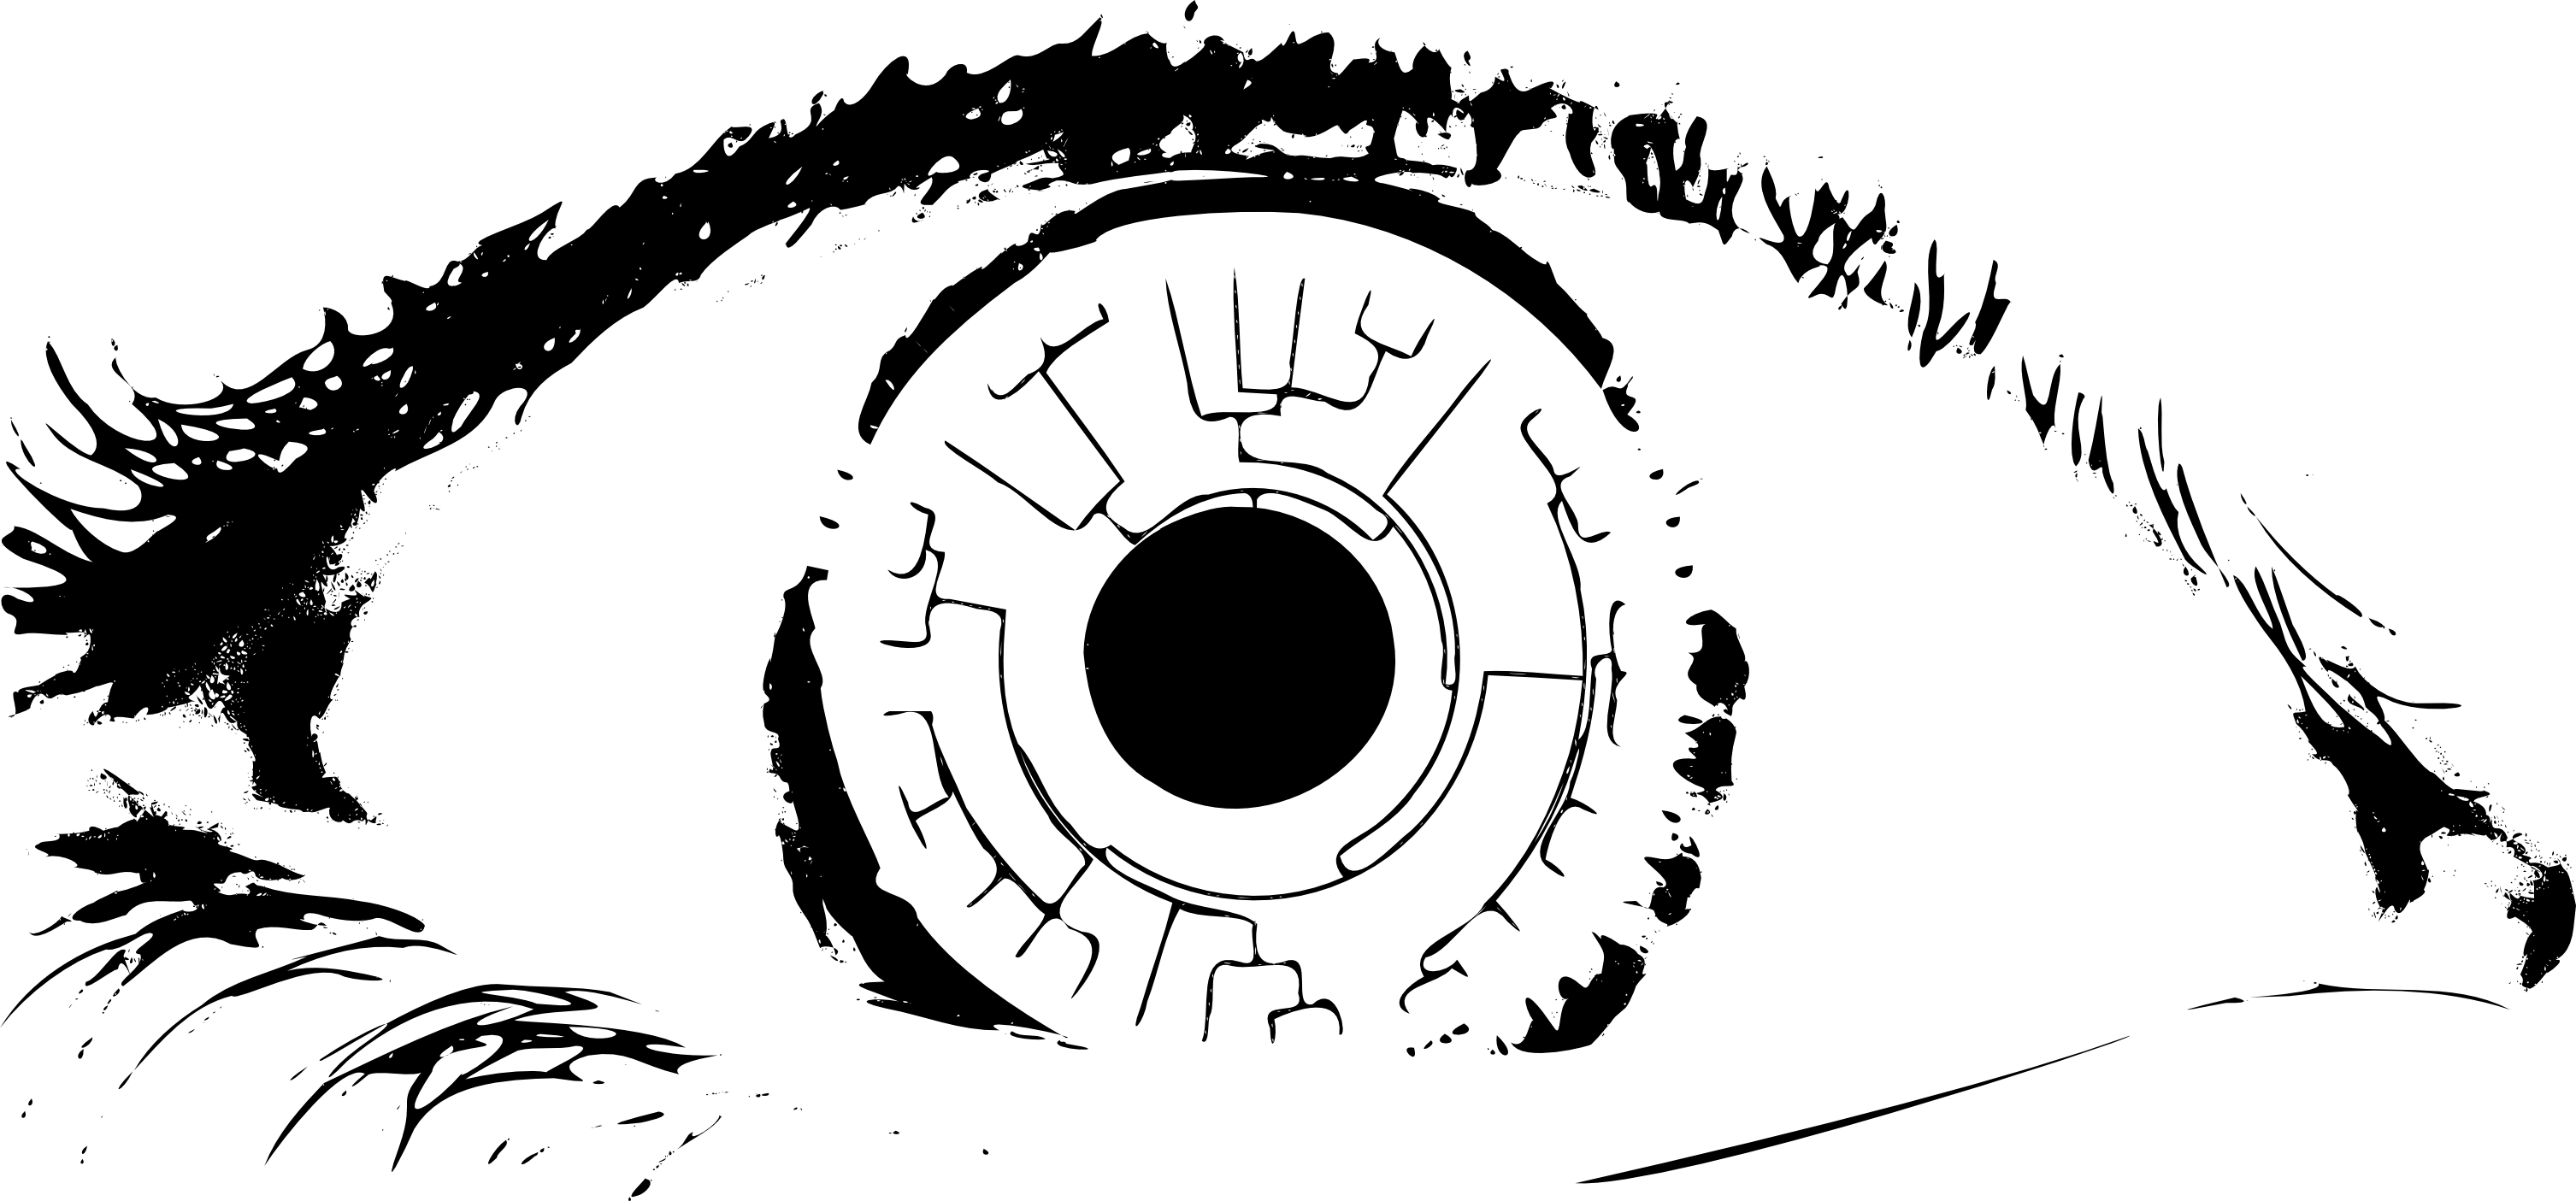
\includegraphics[width=.45\textwidth]{ch2-time/eyepic.png}
\end{figure}

\begin{quoteshrink}
  ``Time is an illusion. Lunchtime doubly so.''

\hfill{Douglas Adams}
\end{quoteshrink}

%%And suddenly I realised that I was no longer driving the car consciously. I was driving it by a %%kind of instinct, only I was in a different dimension.
%% Ayrton Senna


\begin{abstract}
Body size and metabolic rate both fundamentally constrain how species interact with their environment. While many mechanisms leading to these constraints have been explored, their effects on the resolution at which temporal information is perceived have been largely overlooked. The visual system acts as a gateway to the dynamic environment and the relative resolution at which organisms are able to acquire and process visual information is likely to restrict their ability to interact with events around them. As both smaller size and higher metabolic rates should facilitate rapid behavioural responses, we hypothesized that these traits would favour perception of temporal change over finer timescales. Using critical flicker fusion frequency, the lowest frequency of flashing at which a flickering light source is perceived as constant, as a measure of the maximum rate of temporal information processing in the visual system, we carried out a phylogenetic comparative analysis of a wide range of vertebrates that supported this hypothesis. These results have implications for the evolution of signalling systems and predator-prey interactions, and, combined with the strong influence that both body mass and metabolism have on a species' ecological niche, suggest that time perception may constitute an important and overlooked dimension of niche differentiation.
\end{abstract}

\section{Introduction}

All biological systems, from organisms to ecosystems, are shaped by universal constraints. For example, body size and metabolic rate are both known to be important determinants of aspects of organism biology such as life history, energetics and behaviour \citep{brown2004, woodward2005, sibly2012metabolic}. More recently the fundamental role of sensory biology in ecological interactions has gained attention such as research on the limitations imposed on target identification and the scaling allometry of sensory organs \citep{howland2004allometry,cronin2005role,garamszegi2002coevolving}. Such sensory limitations can heavily determine ecological interactions through, for example, predation and mate selection were the abilities of the parties involved to capture, escape or be seduced is dependent on how they perceive their environment (Fig. 1; \citealt{cronin2005role,clark2012field,hornstein2000sexual,stevens2007predator}). While the ability and importance of an organism to perceive the spatial dimensions of its environments are relatively well studied (\citep{cronin2005role,clark2012field}, classic citation on spatial perception Frog targeting?), how they perceive the 4th dimension, time, is less well known.

As the environment is fundamental dynamic in nature the ability to integrate information over timescales is a necessity for any organism interacting within it. The ability to integrate information over shorter timescales, that is, at higher resolutions, is thus a direct limitation on the degree to which it can interact with the environment itself. Furthermore, temporal resolution is also directly linked to the perception of the passage of time itself for humans, in particular when tracking fast moving stimuli \citep{hagura2012ready}. From an evolutionary perspective this leads to a trade-off between the demand for information at high temporal resolution and the costs of its acquisition given the energetic demands associated with increased rates of neural processing in the visual system \citep{laughlin2001energy}. This trade-off is likely to be shaped by various ecological (e.g. mode of predation) and environmental factors (e.g. light levels) as well as intrinsic factors (e.g. morphology) that will ultimately shape an organism's optimal temporal resolution for sensory perception. For example, predators of slow-moving prey may require less temporal resolution than predators that engage in active pursuit of fast-moving prey, such as raptors catching prey during flight.

\begin{figure}[h]
  \centering
  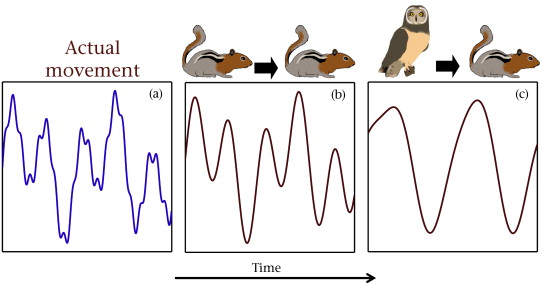
\includegraphics[width=.95\textwidth]{ch2-time/Figure_1.jpg}%Note that this is the path for the folder
  %for chapter 2 that has the Tastes_funny.jpg file within it.
  \caption[Figure 1.]{ The ability of an organism to track a moving object depends on the time integral over which the individual can obtain its information. This is determined by its ability to resolve temporal information. In cases where an animal, such as a ground squirrel, displays complex movement (a), conspecifics may perceive the individual as moving according to a first-order integral of its actual movement owing to its high temporal resolution abilities (b). However a species with lower temporal resolution abilities, such as a short-eared owl, may perceive the motion as an even higher order derivative of the actual motion, meaning information of prey motion at finer temporal scales is not available to it (c).}
  \label{fig:Figure 1.}
\end{figure}


This ability to perceive and react to a dynamic environment is a key behavioural and ecological trait. Ecologically, interaction strengths can be affected by the ability to identify and track fast-moving objects such as prey or mates (Fig. 1; \citealt{land1974chasing, fritsches2005warm}. The necessity of this ability to perceive one's environs accurately is perhaps best demonstrated in cases where temporal resolution is too coarse to allow the observer to follow the motion of a moving target accurately. A stark demonstration of this can be seen in the tiger beetle, Cicindela hudsoni, which, owing to the relatively low temporal resolution of its visual system, must take a stop-start approach in order to recalibrate the position of its prey when hunting \citep{gilbert1997visual}. In humans, the limitations of our temporal perception are apparent when tracking fast-moving objects such as the curving trajectory of a ball in soccer \citep{dessing2010bending} and baseball \citep{bahill2004rising}.

Two intrinsic factors that may shape the costs and benefits of the temporal resolution of the sensory system, in particular with respect to their effects on an individual's ability to interact with the environment on short timescales, are body size and metabolic rate. As larger body sizes decrease manoeuvrability \citep{heglund1988speed,dudley2002mechanisms,biewener2003animal,sato2007stroke,vogel2008modes,hedrick2011damping,watanabe2012slowest} and higher metabolic rates increase both manoeuvrability and the physiological ability to process information \citep{li2008optimal,franz2002temperature}, we hypothesized that smaller organisms and those with higher metabolic rates perceive temporal change on finer timescales.

To quantify the temporal perceptual abilities of a range of species we took advantage of the all or nothing nature of neural firing in the visual system. Owing to this binary firing, temporal resolution must be encoded in terms of discrete units, as biological visual systems must discretize the continuous-time and continuous-space information reaching the retina and then integrate this information over some time period. This "integration time" of visual systems can be quantified using the critical flicker fusion frequency (CFF): the lowest frequency of flashing at which a flickering light source is perceived as constant \citep{d1998can,schwartz2010visual}. As light intensity can increase the number of flashes that can be observed per second, the maximum CFF value, as measured in a response curve of CFF against light intensity \citep{ferry1892persistence,porter1902contributions}, can be used as a proxy for the temporal resolution of the sensory system.

We used CFF to compare the temporal resolution of the visual system in a wide range of vertebrate species including representatives from Mammalia, Reptilia, Aves, Amphibia, Elasmobranchii and Actinopterygii. Using phylogenetic comparative methods and controlling for the light levels each species typically experiences, we tested whether the temporal resolution of the sensory system increases with mass-specific metabolic rate and decreases with body mass.

\section{Methods}
\subsection{Data Collection}
To test our prediction that CFF increases with mass-specific metabolic rate and decreases with body size (when controlling for light levels), we collated data on CFF values of vertebrate species from the literature (Table 1). We only included values from studies that measured CFF using either behavioural or electroretinogram (ERG) procedures. In behavioural studies, CFF is measured through conditional training with the subject trained to respond to a change in its perception of a flashing light \citep{d1998can,rubene2010presence}. For example, \citep{lisney2011behavioural} conducted behavioural tests in domestic chickens, \textit{Gallus gallus}, using choice experiments with flickering and non-flickering stimuli windows with choice of the correct stimulus rewarded with food. This is repeated over a range of light intensities and flicker frequencies until individuals can no longer distinguish between the stimuli. In ERG studies, a direct measurement of the electrical response in the retina in reaction to a flashing light source is used as a measure of CFF \citep{d1998can,schwartz2010visual}. As there may be further processing of temporal information after it reaches the retina that may cause behavioural studies to measure lower CFF values \citep{d1998can}, we included the experimental procedure used to measure CFF as a candidate covariate in our models. We also noted whether each study was a reliable measure of the maximum possible CFF. As maximum CFF is a function of many variables, such as light intensity, and not all studies reported a sufficient range of intensities, their reported CFF may not be the "true maximum" possible. To ensure this did not affect our results we ran an additional analysis that included a term based on this assessment as a categorical covariate as part of our sensitivity analyses (see Appendix).
%changethe end of that to less weak response

We used mean body masses (g) published in the literature and in databases including FishBase \citep{froese2012fishbase} and Animal Diversity Web \citep{myers2006animal} for each species as the measure of body size. For metabolic rates we used mass-specific resting metabolic rate as measured by oxygen consumption through ventilation in studies in which the subjects were fasted prior to the measurement. We converted these values to W/g using the conversion of 20 J/ml of oxygen consumption \citep{makarieva2008mean} to allow comparison among species. For ram-ventilation species (which require constant movement to force fluid over the respiratory organs), such as sharks and tuna, the resting metabolic rate was taken as the fitted line of oxygen consumption with swimming speed extrapolated to the intercept (swimming speed = 0 m/s; Table 1). To account for the possible effect of metabolic rate measured at different temperatures in ectothermic species, metabolic rate values were corrected to 20 $^{\circ}$C using Q10 values, i.e. the fold change in metabolic rate over a temperature change of 10 $^{\circ}$C, for reptiles, amphibians and fish \citep{white2006scaling}. These corrections gave values of temperature-corrected mass-specific resting metabolic rates (qWg), for each species. Although body mass and mass-specific metabolic rate are expected to be correlated according to an exponent of 0.25 \citep{brown2004, sibly2012metabolic} (Brown et al., 2004 and Sibly et al., 2012), we included both terms as recommended by \citep{freckleton2009seven} instead of using residuals from a regression of body mass against mass-specific metabolic rate.

As there is a trade-off between sensitivity and movement perception owing to the requirement of longer integration times in low light conditions \citep{tansley1965vision}, as is seen in the different light response dynamics of rods and cones \citep{rubene2010presence}, we included light levels within our analyses as a categorical variable based on the light conditions experienced by the species during normal activity (i.e. foraging). Species were categorized as inhabiting either high or low light conditions with diurnal terrestrial and nonturbid aquatic species coded as inhabiting high light level environments and nocturnal species coded as inhabiting low light levels. As the light levels of species that inhabit turbid waters are typically orders of magnitude lower than typical daylight levels (40-1000 lx; \citealt{ali1985vision,palmer2010art,kreysing2012photonic} and the harp seal, Pagophilus groenlandicus, regularly forages at depths greater than 200m \citep{folkow2004distribution} where light levels are comparable to nocturnal light levels (Palmer and Grant 2010), we categorized these species as inhabiting low light level environments.


\begin{figure}[h!]
  \centering
  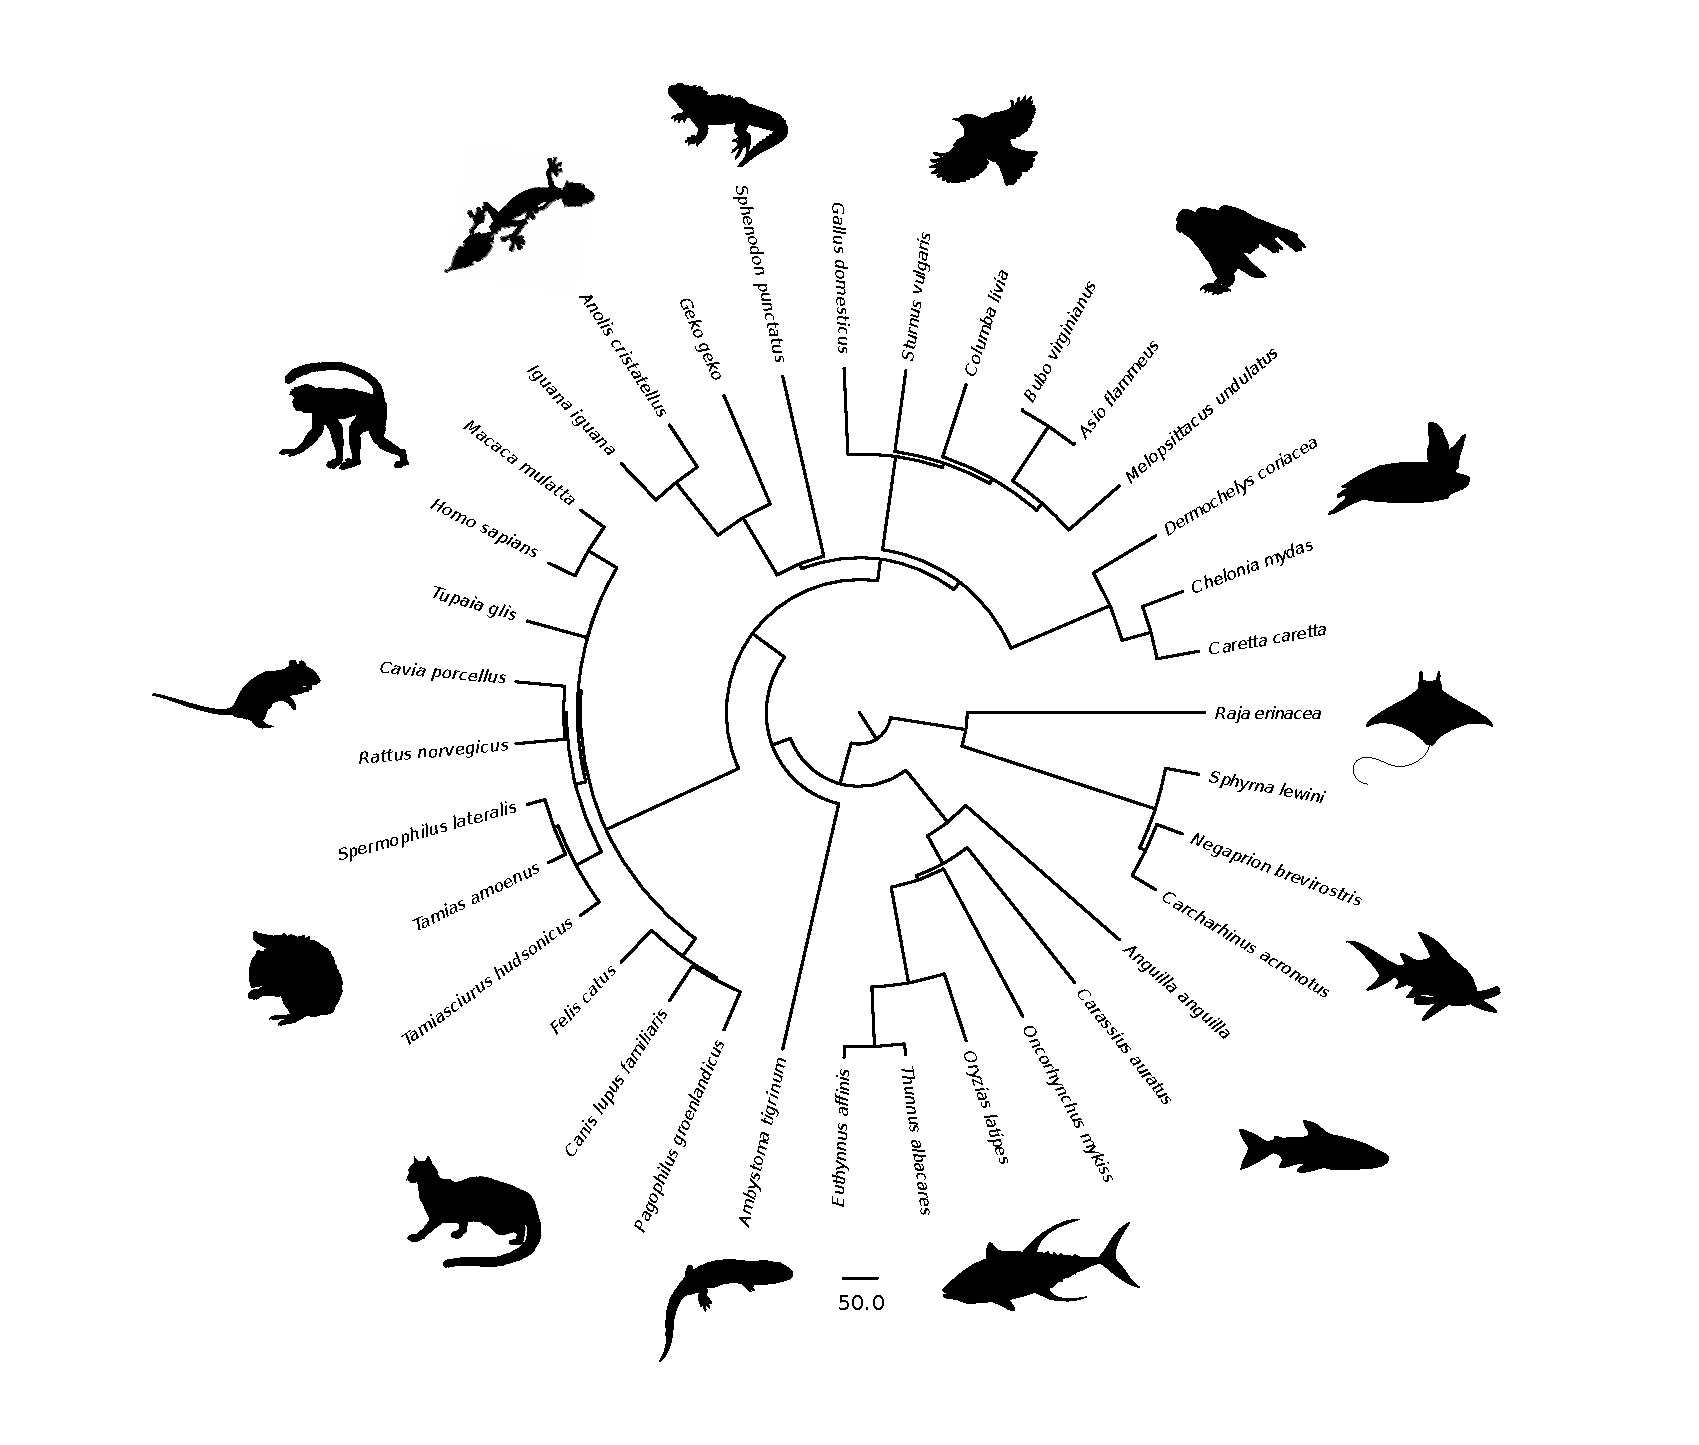
\includegraphics[width=.95\textwidth]{ch2-time/phylofig.pdf}%Note that this is the path for the folder
  %for chapter 2 that has the Tastes_funny.jpg file within it.
  \caption[Figure 2.]{ Composite tree of the study species.}
  \label{fig:Figure 2.}
\end{figure}


To correct for the phylogenetic nonindependence of species we constructed a composite tree of the study species using published molecular phylogenies and divergence times from various sources \citep{schoch1985preliminary,janossy2011pleistocene,mercer2003effects,hedges2006timetree,wiens2006does,benton2007paleontological,murphy2007using,brown2008strong,li2008optimal,naro2008evolutionary,albert2009effect,lim2010phylogeny,little2010evolutionary,perelman2011molecular} (Schoch, 1985,; see the Appendix and Fig. A1). In instances in which a divergence time was not available for two species we used the conservatively estimated date of first appearance as the divergence time taken from the Paleobiology Database \citep{alroy2008phanerozoic}.



As ectotherm metabolic rates vary with temperature, we performed a sensitivity analysis to test the effect of the temperature to which qWg was corrected to by rerunning the main analysis with qWg corrected to both 5 °C and 35 °C (see Appendix). We also carried out a supplemental analysis on a more restricted data set for species with available brain mass data to test for any possible effects of sensory tissue on maximum CFF values (see Appendix).

In total we collected data on maximum CFF, body mass, qWg and light environments for 34 species across the vertebrate classes Elasmobranchii, Actinopterygii, Aves, Amphibia, Reptilia and Mammalia, with further data on brain mass for 28 of these species (Table 1).

\subsection{Statistical Analyses}
To test our hypothesis we used a phylogenetic generalized least-squared approach (PGLS) using the caper package \citep{orme2011caper} in R version 2.14.2 \citep{RCran}. The PGLS approach is based on standard generalized least-squared models while also accounting for the nonindependence in the data caused by species' phylogenetic relationships by incorporating it through the error term structure \citep{pagel1999inferring,rohlf2001comparative}. This error term consists of a matrix of expected trait covariances calculated using the maximum likelihood estimate of lambda (), a multiplier of the off-diagonal elements of a phylogenetic variance–covariance matrix that best fits the data. When the data are structured according to a Brownian motion of trait evolution, lambda = 1, whereas when the data have no phylogenetic dependency, then lambda = 0 \citep{pagel1999inferring}.

We ran PGLS models with maximum CFF as the response variable, and all combinations of the following explanatory variables: body mass, qWg, light level (high, low) and experimental procedure (ERG, behavioural) with brain mass and methodological optimality included in the sensitivity analysis (see Appendix). We did not include interactions, as there was no a priori reason to include them. We used the Akaike information criterion (AIC), which penalizes extra effective parameters to avoid overparameterized models, to select the minimum adequate model \citep{burnham2002model}.


\begin{table}[h!]
  \caption[Table 1.]{Data used in analysis}
  \label{tbl:Table 1.}
  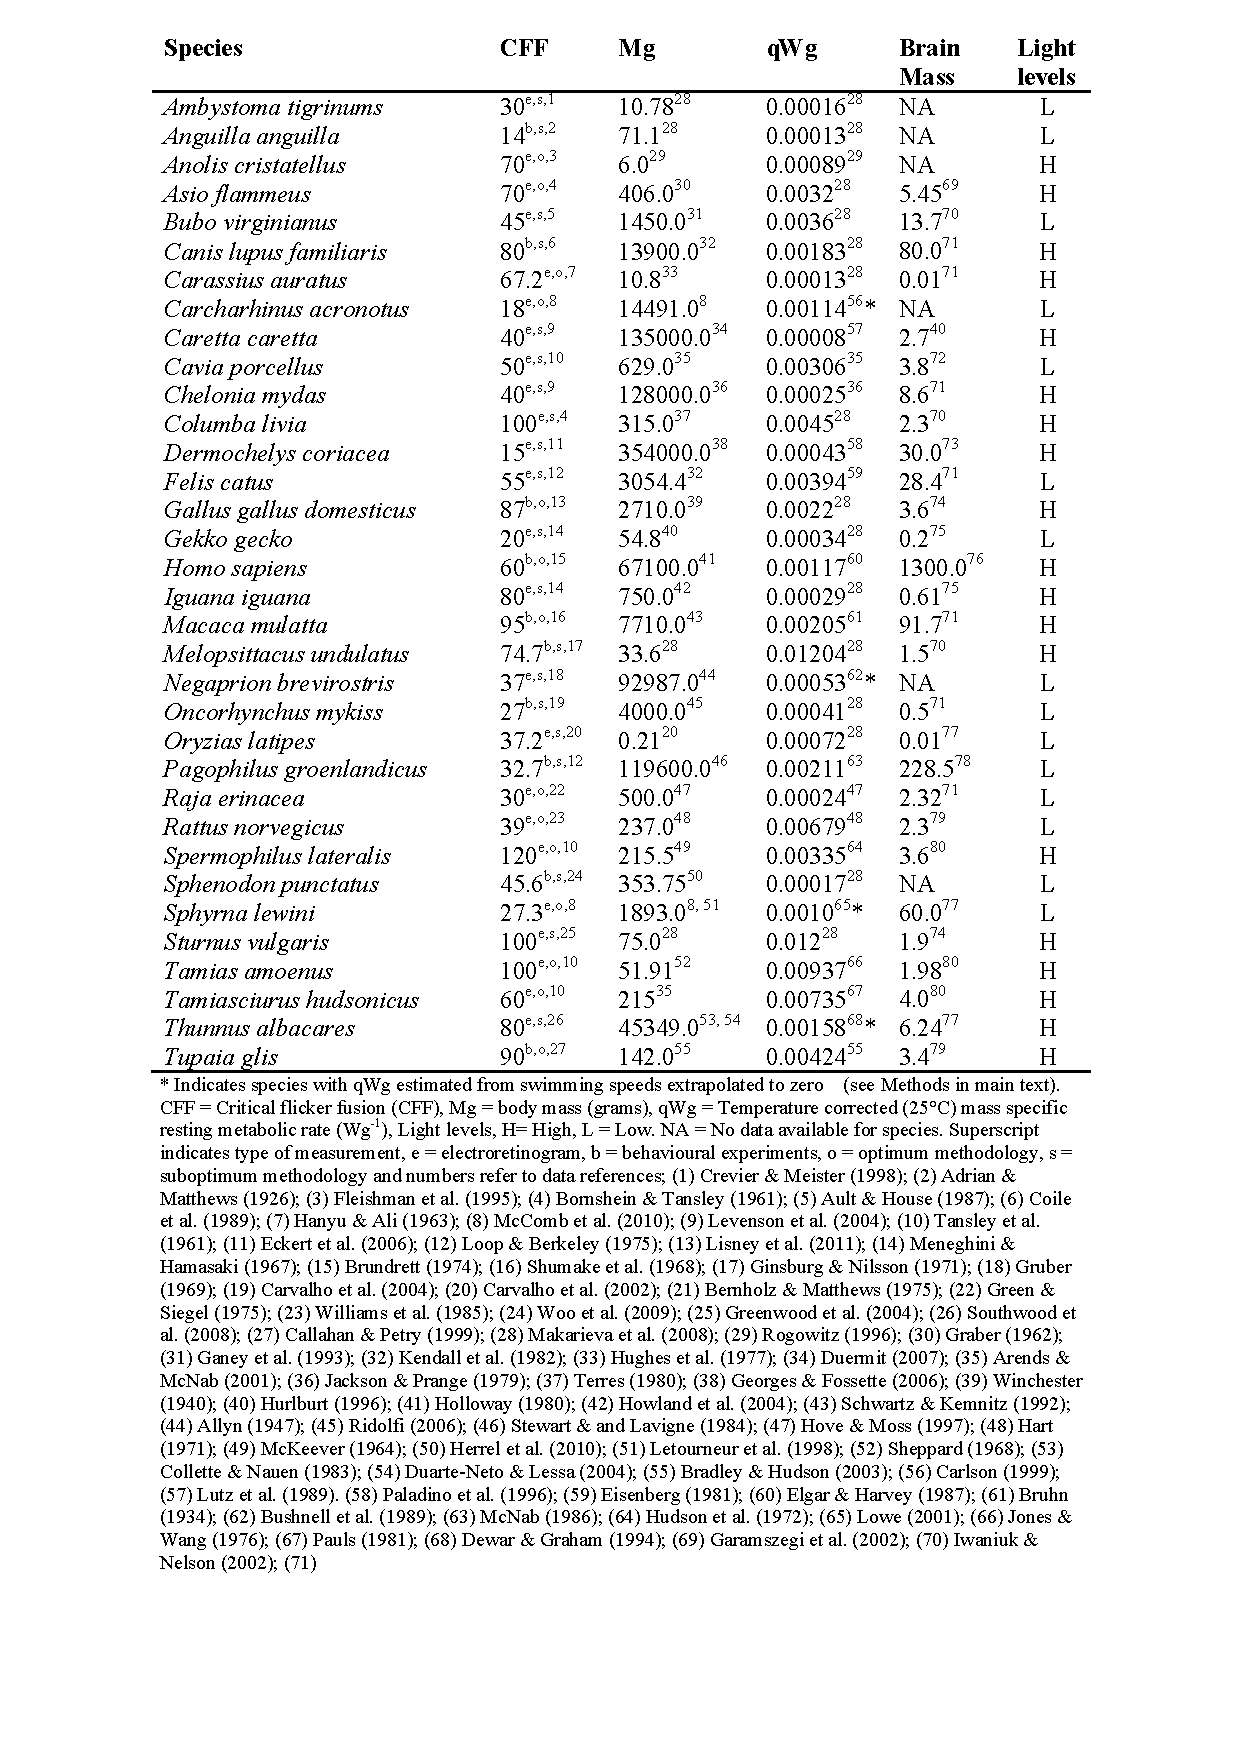
\includegraphics[width=\linewidth]{ch2-time/Table_1}
\end{table}


\section{Results}
The most parsimonious model (based on AIC) explaining variation in maximum CFF among vertebrates included the terms body mass, temperature-corrected mass-specific resting metabolic rate (qWg) and light level (Table 2, Tables A1 and A5 in the Appendix). The second most parsimonious model, which fell within two AIC values of the most parsimonious model, retained all tested variables (Table 2). Body mass had a negative effect on the temporal resolution of the sensory system (Table 2, Fig. 2a, Fig. A2 in the Appendix), with a change in body mass of approximately 10 kg resulting in a reduction in CFF of 2 Hz. The metabolic rate of organisms, after correcting for mass, was positively associated with CFF while low environmental light levels were associated with an overall reduction in CFF (Table 2, Fig. 2b, Fig. A2 in the Appendix). Phylogeny was found to have a minimal effect on the resulting models (λ = 0, Table 2) and experimental type was not correlated with CFF (Table 2). Thus, according to our model, small animals with high mass-specific metabolic rates in high light environments possessed the highest maximum CFF and hence greatest ability to perceive temporally dynamic visual information. Conversely, large animals with low mass-specific metabolic rates in low light environments had the lowest CFF.


\begin{table}[h!]
  \centering
    \caption[Table 2.]{Coefficients of the model with all factors included. Mg = body mass (grams), qWg = Temperature corrected mass-specific resting metabolic rate Wg-1, Light.l (low) = effect of low light levels on CFF in comparison to high light levels, exp = effect of experimental type (ERG = electroretinogram) in comparison to behavior based CFF measures.}

\begin{tabular}{*5l}    \toprule
\emph{Variable} & \emph{Estimate} & \emph{S.E} & \emph{t-value}&  \emph{P-value}\\\midrule
Intercept    & 141.48  & 15.15  & 9.34  &  {\ensuremath{4^{-10}}}\\ 
Mg & -4.40 & 2.01 & -2.18 & 0.038\\
qWg & 16.89 & 4.31 & 3.92 & {\ensuremath{5^{-4}}}\\
Light levels (low) & -37.74 & 5.94 & -6.36 & {\ensuremath{7^{-7}}}\\
Measurement type (exp) & -3.66 & 6.24 & -0.59 & 0.56\\
Data quality (high) & -3.86 & 6.14 & -0.63 & 0.53\\
 &  & & & \\
 & Mode & Lower 95\% C.I & Upper 95\% C.I\\ 
Lambda  (Low) & 0 & 0 & 0.34 &\\
&  &  &  &{\ensuremath{R^2}= 0.69}\\\bottomrule
 \hline
\end{tabular}
  \label{tbl:Table 2.}
\end{table}


These results were robust to our sensitivity analysis on both the temperature used to correct ectotherms qWg (taken as 25 °C in the main models above; see Methods) and the optimality of study methodology for measuring maximum CFF, with the best models in both sensitivity analyses (based on AIC) including the same terms and trends as found in the main analysis (Tables A2, A3, A5, A6, A7 and A9 in the Appendix). We also found that including brain mass in a restricted data set of 28 species for which brain mass was available did not change the effect of the explanatory variables light levels, qWg and body mass on maximum CFF (Tables A4 and A8 in the Appendix).


\begin{figure}[h!]
  \centering
  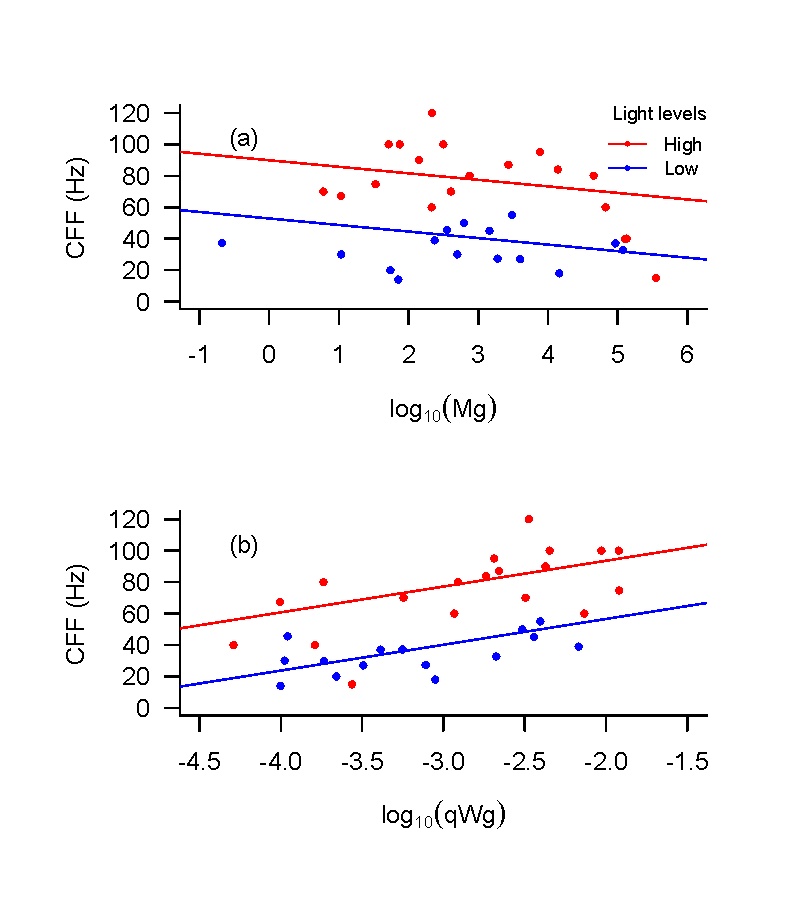
\includegraphics[width=.95\textwidth]{ch2-time/Figure_2}%Note that this is the path for the folder
  %for chapter 2 that has the Tastes_funny.jpg file within it.
  \caption[Figure 3.]{ The effect of  log body mass, light levels and log temperature corrected mass-specific resting metabolic rate (qWg) on critical flicker fusion frequency (CFF). The minimal adequate model (Results) indicates CFF increases with log qWg but decreases with body mass. Low light levels (blue) are associated with low CFF values in comparison to high light levels (red).}
  \label{fig:Figure 3.}
\end{figure}


\section{Discussion}
Many of the interspecific and intraspecific interactions that shape species' behaviour and ecology rely on the ability of organisms to process high temporal resolution sensory information. Our results show that, while there is considerable variability in the ability to resolve temporally dynamic visual information across vertebrates, body mass and metabolic rate act as important general constraints on this ability. This is the first study to indicate a general trend in the ability of vertebrates to resolve temporal information; previous studies have generally focused on specific cases of sensory adaptations \citep{fritsches2005warm} and particular environments \citep{frank1999comparative,frank2012light}, hence focusing on the particular ecological context of each adaptation or environment. Our findings illustrate the relationship between both physiology and the effects of body mass on the ability to resolve temporal features of the environment on fine timescales, hence linking sensory adaptations to fundamental constraints and trade-offs imposed on all organisms.

\cite{autrum1958electrophysiological} hypothesis, that the response dynamics of the retina should be shaped by the organism's particular ecology, predicts that organisms that demand fast visual systems will acquire adaptations increasing CFF values, and hence temporal resolution. This can be achieved through alterations to the rate of neuron firing, a fundamental limit to the rate of information transfer, through the provision of energy \citep{laughlin2001energy} or changes in the physiological environment. For example, blowflies \citep{tatler2000temperature} and predatory swordfish \citep{fritsches2005warm} both use specialised heating tissues that increase the temperature, and hence the metabolic rate, in their visual systems, which in turn up-regulates their CFF. Similar adaptations are also seen across species of large, fast-swimming predatory billfish \citep{carey1982brain} and Lamnidae sharks \citep{block1985warm}. Physiological adaptations for high-resolution motion detection are also found within specific areas of the retina in some flies, commonly referred to as the "love spot", which allow them to identify female flight patterns accurately and thus detect mates \citep{land1974chasing}.

In a broader context, it might be expected that manoeuvrability, a vital component of an individual's ability to respond to the environment, may be one of the main factors determining whether it is necessary to invest in costly temporal information processing. Manoeuvrability, as defined by the ability to change body position or orientation, generally scales negatively with body mass. This negative scaling emerges primarily through the increased inertia and decreased limb stroke rate associated with large body size in both aquatic and volant species \citep{dudley2002mechanisms,sato2007stroke,vogel2008modes,hedrick2011damping,watanabe2012slowest}, while in terrestrial species changes in gait posture that redistribute weight across the limbs can explain such reduced manoeuvrability with body mass \citep{heglund1988speed,biewener2003animal}. These arguments show that, owing to the laws of physics, larger animals physically respond less quickly to a stimulus. Hence we expect selection against costly investment in sensory systems with unnecessarily high temporal resolution in large animals, as information on such timescales can no longer be utilized effectively. This may explain why larger vertebrates, along with those with low metabolic rates, had lower temporal resolution in our study. This idea is also supported by research showing that faster and more manoeuvrable fly species have higher temporal resolutions \citep{laughlin1993fast} and that less manoeuvrable scavenger crabs display slower response dynamics than deeper living predatory species which are likely to have more active lifestyles \citep{frank2012light}.


While many species have evolved adaptations to overcome sensory limitations most species in our results conform to a general scaling in their temporal ability. Hence while body size and metabolic rate are known to good proxies to the rate which individuals can interact with the environment we show that this proxy also extends towards perceptual abilities. Hence while a individual may be theoretically capable of interacting with another individual, its inability to track its movement or fully process a signal may practically excuse it form the interaction.


The effects of body size and metabolic rate on temporal resolution and the presence of sensory adaptations, as discussed above, also point towards an interesting dimension of niche space. Disparity in size and metabolic rate among species within an ecological setting may select for particular sets of adaptations creating a diverse set of sensory systems and interactions. In such a system, species might occupy the same spatial and temporal niche, but could be separated owing to differential responsiveness to environmental signals and cues as a result of having evolved divergent signalling systems along a dimension represented by temporal resolution. For example, it seems at least theoretically possible to encode information in high-frequency signals that can be detected by intended receivers such as conspecifics but that are not susceptible to "eavesdropping" by (generally larger) predators. Ecological systems in which this may be apparent include deep-sea systems where visual signalling is an important determinant of the ability of organisms to interact, and where bioluminescence flashing over wide frequency ranges is ubiquitous \citep{haddock2005bioluminescent,widder2010bioluminescence}.


Overall our results show that not only are body size and metabolic rate good proxies for the rate of biological interactions they are good proxies for the ability to perceive such interactions. While interaction rates are strongly coupled with the spatial dimensionality of the environment and searching rates associated with them \citep{pawar2012dimensionality} the temporal dimension in which an individual resides will also strongly influence its ability to interact with that environment. The generality of these findings suggest that temporal resolution may play a much more important role in sensory ecology than previously indicated, in particular because of its universal effects relating to body size. Further investigations into both the underlying mechanisms of these findings and their importance to ecological functioning are needed.


\bibliographystyle{PLoS-Biology}
\bibliography{bibfile}

	%This is a ch2-labstudy.tex file with contents of intro chapter etc.
\chapter[Longevity]{Ecology and mode-of-life explain lifespan variation in birds and mammals}
\label{chap:Longevity}


\begin{figure}[h]
  \centering
  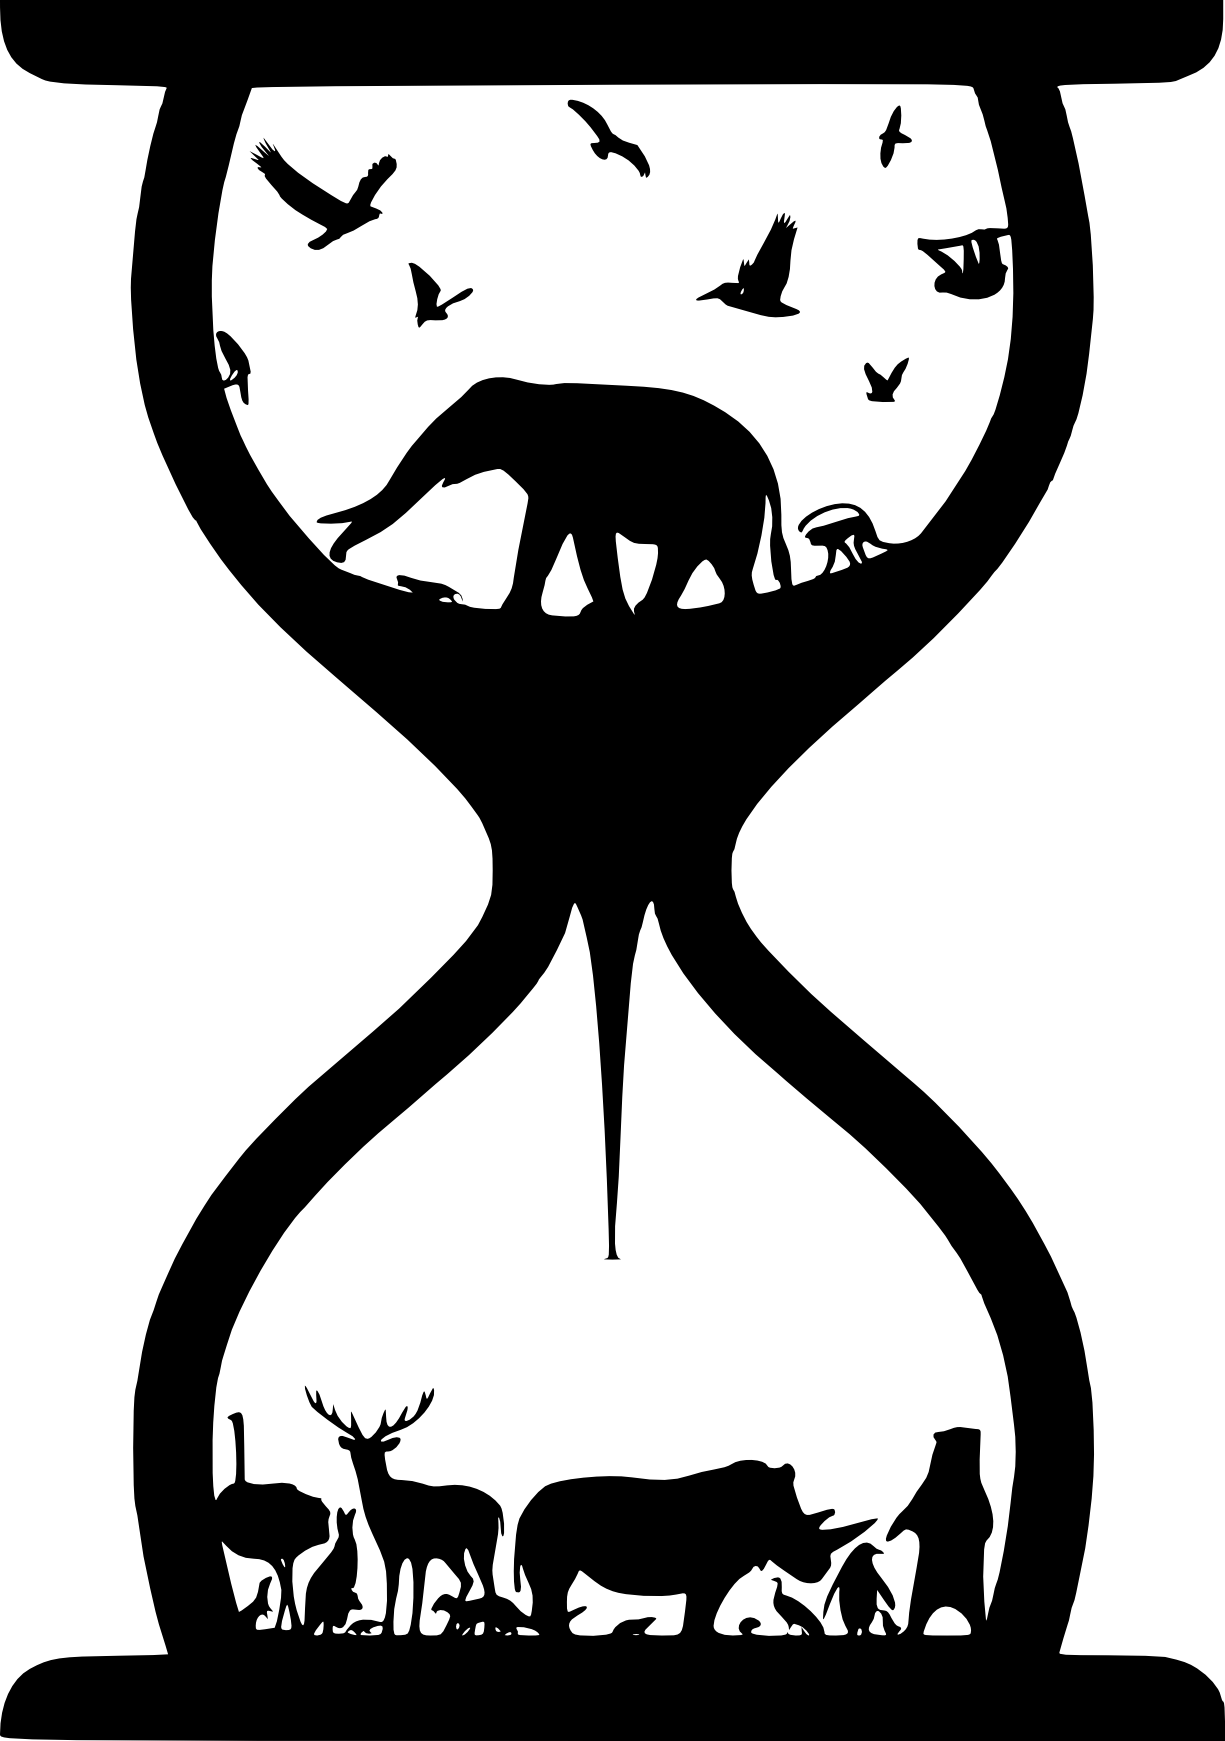
\includegraphics[width=.20\textwidth]{ch3-longevity/long.png}
\end{figure}


\begin{quoteshrink}
  ``Achieving life is not the equivalent of avoiding death.''
  
\hfill{Ayn Rand}
\end{quoteshrink}

%%%%%Always keep your smile. That's how I explain my long life. Jeanne Calment



\begin{abstract}
Many species live far longer than expected given their body mass. This may reflect interspecific variation in extrinsic mortality, with species capable of reducing mortality expected to exhibit longer lifespans. One such factor that may strongly influence such extrinsic mortality is habitat dimensionality. As higher dimensional habitats create multiple escape routes from predation, species associated with such environments would be expected to have higher maximum lifespans. Here, I investigate how such traits associated with habitat dimensionality inducing volancy, arboreality and fossoriality, along with other potential traits, including activity patterns and eusociality, influence lifespan across birds and mammals. Using phylogenetic comparative analyses with over 1300 species I show that, over and above the effect of body mass, species associated with high dimensional habitats, through arboreality and the ability to fly, live the longest. Within volant species, lifespan depended upon when (activity patterns), but not where (foraging habitats), species are active. However, the opposite was true for non-volant species, where lifespan correlated positively with both arboreality and whether they were eusocial. These results indicate that dimensionality can affect the ability of prey to escape predation with the resulting affects on species life-history evolution. 

\end{abstract}

\section{Introduction}

Lifespan, or longevity, is a fundamental life-history trait that exhibits considerable variation both within and among species. Maximum lifespan in vertebrates, for example, ranges from up to 211 years in the bowhead whale (Balaena mysticetus;\citep{de2009database}), down to just eight weeks in the pygmy goby (Eviota sigillata; \citep{depczynski2005shortest}). Like most other life-history traits, lifespan varies strongly with body size such that large species tend to live longer than smaller species \citep{lindstedt1981body,promislow1993size,de2007analysis,ricklefs2010life}. However, many species have far longer, or indeed shorter, lives than expected given their body mass (Figure 1). Understanding the mechanisms underlying these deviations from predicted lifespan may reveal the secrets to treating and combating human ageing \citep{ricklefs2010insights,zhang2013comparative}. 

One explanation for species living longer than expected, given their body size, is that low extrinsic mortality (i.e. low risk of death due to external causes such as disease, predation, food shortages  or accidents) will, on average, select for longer lifespans than when extrinsic mortality is high \citep{stearns1992evolution,Williams1957}. This is because when untimely death is more likely, investment in early and frequent reproduction is favoured rather than investment in long-term maintenance and survival. Therefore, species with adaptations that reduce the risks of extrinsic mortality should live longer than expected, given their body mass \citep{partridge1993optimality}. These ideas have led to myriad, taxon-specific hypotheses about traits that may reduce extrinsic mortality and result in increased lifespan (reviewed in \cite{ricklefs2010insights}). However, there is little consensus about the general drivers of increased lifespan across clades.

As predation is one of the main sources of extrinsic mortality, species which possess the ability to reduce it, for example through the use of toxin defences, show increased lifespans [ref]. One fundamental ecological aspect that would be expected to affect such predation pressures is the dimensionality of the habitat a species lives within. The dimensionality of trophic interactions is a key element in predation pressures where consumption rates scale higher with body mass in high dimensional interactions \citep{pawar2012dimensionality}. While this increased scaling of potential predation pressures may be expected to decrease prey species longevity in such environments the converse may also be expected through the increase ability of prey species to escape due to the increased availability of escape routes in terms of directionality and cover. Two such common ways a species may access such escape paths include arboreality and the ability to fly.

The ability to fly, and thus more easily escape predation and unfavourable conditions, is perhaps the most effective way a terrestrial species can evolve to reduce its extrinsic mortality and increase its lifespan \citep{partridge1993optimality,holmes1994fly,pomeroy1990fly}. This is supported strongly by striking differences in the lifespan of volant (flying) and non-volant (non-flying) vertebrates; on average, bats live 3.5 times longer than similarly-sized non-volant placental mammals \citep{wilkinson2002life,austad1991mammalian}, while birds live up to four times longer than similarly sized mammals \citep{lindstedt1981body,holmes2003birds}. Similarly aeboeriality has also been cited as extending longevity in species mainly through decreasing predations risks \citep{shattuck2010arboreality}. However, these may not be the only route to reducing extrinsic mortality and thereby increase lifespan. Ecological factors may also be important. Previous studies have investigated the relationship between lifespan and various ecological variables, but most only investigated select groups of species and few considered multiple traits simultaneously (e.g. \cite{shattuck2010arboreality}).

Here I investigate how multiple ecological and mode-of-life traits simultaneously influence maximum lifespan across birds and mammals. I test several hypothesis regarding the relationships among lifespan and ecological and mode-of-life traits known to influence extrinsic mortality risk; including flight capability (volant or non-volant), activity period (diurnal, crepuscular [i.e. active at dawn and dusk], nocturnal or cathemeral [i.e. active both day and night]), foraging environment (terrestrial, semi-arboreal, arboreal, aerial or aquatic), and fossoriality (i.e. living in burrows; fossorial, semi-fossorial, non-fossorial). I approach these questions by using the largest number of species to date in such an analysis (N =  589 birds and 779 mammals) and by using the most up to date phylogenetic comparative approach that includes using a distribution of 500 combined bird and mammal phylogenies to control for the phylogenetic autocorrelation introduced by shared ancestry \citep{harvey1991comparative} and body mass \citep{lindstedt1981body}.


I predict that, after controlling for body mass, species which can accesses escape routes within high dimensional habitats including (i) volant and arboreal species will either show reduced or enhanced lifespans in comparison to other species; (ii) semi-arboereal, semi-aquatic and semi-fossorial species which can seek refuge across different environments would be expected to live longer then terrestrial species; Species with nocturnal, crepuscular or cathemeral activity patterns will live longer than diurnal species, because species that are active at night or dusk are likely to be harder for predators to detect \citep{holmes1994fly,promislow1990living}; and (4) fossorial (i.e. species that live in permanent burrows) will live longer than purely terrestrial species, because they possess means to escape predation and unfavourable conditions through refuge \citep{buffenstein2002naked}.

As ecological factors that influence lifespan are likely to vary among volant and non-volant species because sources of extrinsic mortality will differ in these two groups, these groups were split species into volant (most birds and all bats), and non-volant (some birds and most mammals) subgroups, to discover general, broad-scale correlates of lifespan in endotherms, rather than separate correlates for birds and mammals. I then tested the above hypotheses on volant and non-volant species separately. As predicted, after controlling for body mass and phylogeny, volant and arboreal species live longer then terrestrial species. Surprisingly of the species capable of transitioning across environments only semi-arboreal species showed increased lifespan while only volant crespucular species showed any effect of activity period on longevity.

\section{Materials and Methods}
\subsection{Data}

We used maximum longevity as our measure of lifespan as it is thought to be the best available estimator of a species' ageing rate \citep{de2007analysis} and because of the amount of high quality longevity data available. We obtained data on maximum longevity (years) and adult body mass (g) from the AnAge database \citep{de2009database,tacutu2012human}. In our main analysis we excluded species with maximum longevity estimates based on fewer than ten longevity records, or with low or questionable data quality as defined in the AnAge database \citep{de2007analysis}. As maximum values are dependent on sample size we also ran a sensitivity analysis excluding species with maximum longevity estimated from fewer than 100 longevity records. Note that longevity records for non-volant mammals tend to come from captive individuals, whereas data for bats and birds tend to come from wild caught individuals. Although we expect captive individuals to live longer than wild individuals, on average maximum longevity tends to remain unchanged between captive and wild populations \cite{ricklefs2001comparison}. Further, given that bats and birds live longer than non-volant mammals, this should make our analyses more conservative. 

To test our hypotheses concerning the relationships between lifespan, mode-of-life and ecological traits, we collected data on the flight capability (volant or non-volant), activity period (diurnal, crepuscular, nocturnal or cathemeral), foraging environment (terrestrial, semi-arboreal, arboreal, aerial or aquatic), and fossoriality (fossorial, semi-fossorial or non-fossorial) of each species using Walker's Mammals of the World \citep{nowak1999walker}, the Handbook of Birds of the World series \citep{hoyo1992handbook}[25], the Handbook of the Birds of Europe, the Middle East and North Africa series \citep{cramp1977handbook} and some additional sources (Appendix 1, \citep{fry2010kingfishers,parr2010parrots,williams1995penguins}). These categories are described in detail in Appendix 1. We used the taxonomy of Wilson and Reeder \citep{wilson2005mammal} for mammals and Jetz et al. \cite{jetz2012global} for birds. We excluded purely aquatic mammals (Cetacea and Sirenia) from the analyses because we expect selection pressures to be very different in these groups. We also excluded gliding mammals because there were too few species (N = 9) to run a separate analysis and because this group could equally fit into either the volant or non-volant subgroups.

Rather than basing our analyses on just a single phylogenetic tree and assuming this tree was known without error, we instead used a distribution of trees. We extracted 500 bird trees from the posterior distribution of a recent bird phylogeny generated under a Bayesian inference framework \citep{jetz2012global}, and used the 10,000 mammal trees constructed by Kuhn et al. \citep{kuhn2011simple}. Each individual mammal tree comprises one resolution of the polytomies of a previously published supertree \citep{bininda2007delayed}. We treat these as equivalent to a Bayesian posterior distribution of trees because no such tree analysis exists for all mammals. As we needed a distribution of phylogenies containing both birds and mammals, we randomly selected one bird tree and one mammal tree (without replacement) and bound them to make a combined tree. The trees were bound with a root age of 315 million years, corresponding to the fossil calibration for all amniotes, i.e.,  \textit{Archerpeton anthracos} (Appendix 1; \citep{reisz2004molecular}). We repeated this procedure 500 times to generate a distribution of 500 combined bird and mammal trees.

Many studies on vertebrate ageing have noted a strong correlation between maximum longevity and metabolic rate. Opinion is divided as to whether this is a causative relationship or merely confounded with the strong correlation between body mass and metabolic rate \citep{ricklefs2010insights}. To determine whether our conclusions hold when we include metabolic rate in our models, we also compiled mass-specific basal metabolic rate (BMR; Wg-1) data (see Appendix 1).


In total our analyses used data from 589 birds (579 volant and 10 non-volant) and 779 mammals (83 volant and 696 non-volant; see Appendix 3: Table A1 for more details and Appendix 2 for the complete dataset). This was reduced to 112 birds and 330 mammals when we include BMR in our models, and 474 birds and 435 mammals in the sensitivity analysis using only species with 100 or more longevity records.

\subsection{Analyses}

To test our hypotheses we fitted the following three models, with Maximum longevity and Body mass incorporated as continuous variables; Flight capability, Foraging environment, Activity period and Fossoriality as factors and with Body mass:Flight capability representing the interaction between Body mass and Flight capability:


\begin{enumerate}
  \item For all species (N =1368:
Maximum longevity = f(Body mass +  Flight capability + Body mass: Flight capability)
  \item For volant species only (N = 662):
Maximum longevity = f(Body mass + Foraging environment + Activity period)
  \item For non-volant species only (N =706):
Maximum longevity = f(Body mass +  Foraging environment + Fossoriality + Activity period)
\end{enumerate}


All analyses were carried out in R v3.0.2 \citep{RCran}. Maximum longevity and body mass (and BMR, see below) were log10 transformed to correct inherent skewness before being mean centred and expressed in units of standard deviation.
We fitted our models using Bayesian phylogenetic mixed models from the MCMCglmm package \citep{hadfield2010mcmc}, to account for non-independence in species traits introduced as a result of common ancestry \citep{harvey1991comparative}. MCMCglmm uses a Markov chain Monte Carlo estimation approach and accounts for non-independence among closely-related species by including the phylogenetic relationships among species as a random variable. We determined the number of iterations, thinning and the burn-in period for each model run across all trees using diagnostics in the coda package \citep{plummer2006coda} and we checked for convergence between model chains using the Gelman-Rubin statistic, the potential scale reduction factor (PSR), with all models required have a PSR below  1.1 \citep{gelman1992inference}. Following the recommendations of Hadfield \citep{hadfield2010mcmc}, we used an uninformative inverse-Wishart distribution (with variance, V, set to 0.5 and belief parameter, nu, set to 0.002) and a parameter expanded prior, with a half-Cauchy distribution (described by the parameters V = 0.5, nu = 1, the prior mean alpha.mu = 0, and alpha.V = 102, which represents the prior standard deviation with a scale of 10), for the random factor to improve mixing and decrease autocorrelation among iterations. 

As noted above, rather than using one phylogenetic tree and assuming this tree was error free, we instead used a distribution of 500 combined bird and mammal trees and fitted each of our models to each of these trees. We then combined the resulting model outputs to give model estimates which incorporate the error across the 500 trees.  As the posterior outputs of MCMC models are combinable, coefficient distributions were created by amalgamating each coefficient posterior. 

To determine whether our conclusions held when we excluded species with fewer than 100 longevity records or when metabolic rate was included in our models, we repeated models 1-3 with either the reduced dataset of species with 100 or more longevity records or with BMR as an additional linear covariate. We also repeated Models 2 and 3 for birds and mammals (rather than volant and non-volant species) separately to ensure that differences between the volant and non-volant subgroups were due to differences in flight capability and were not simply representing the difference between mammals and birds. We calculated the deviance information criteria (DIC), a hierarchal generalization of AIC, for each bird and mammal paired models and compared it to the paired volant and non-volant models to compare model "fit" of each approach.

Finally, Since publication of this work \citep{healy2014ecology} new analysis performed by \cite{williams2015ecology} outlined the potential importance of eusociality in small mammals associated with fossoriality. The analysis uses the data described above along with new data on eusociality, defined using reproductive skew \citep{williams2015ecology}, to show that eusociality is also a predictor of increased maximum lifespans. To further analysis this composite dataset I used the methods outlined above to investigate the importance of eusociality while controlling for phylogeny and the error within phylogenetic reconstructions.

\section{Results}

The analysis show that volant species live longer than non-volant species of a similar body mass (Table 1, Figure 1). In addition, for a given increase in body mass, the lifespans of volant species (modal slope estimate [after converting from mean-centred values] = 0.25; Table 1) increase significantly more than the lifespans of non-volant species (modal slope estimate [after converting from mean-centred values] = 0.13; Table 1).


\begin{table}[h]
  \caption[Table 1.]{Relationship between maximum longevity (years), body mass (g) and flight capability (volant or non-volant) in 1368 birds and mammals. Estimates are modal estimates from 500 models. Lower CI = Lower 95\% confidence interval from 500 models. Upper CI = Upper 95\% confidence interval from 500 models. Posterior distribution = distribution of estimates from 500 models. Body mass \: Flight capability = interaction between body mass and flight capability.}
  \label{tbl:Table 1.}
  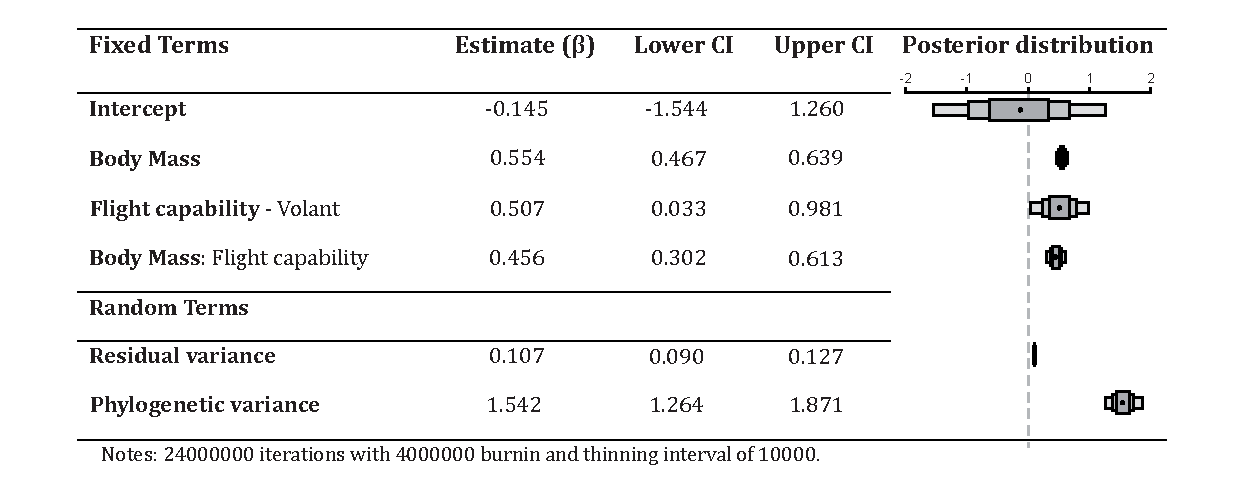
\includegraphics[width=\linewidth]{ch3-longevity/Table1.pdf}
\end{table}


\begin{figure}[p!]
  \centering
  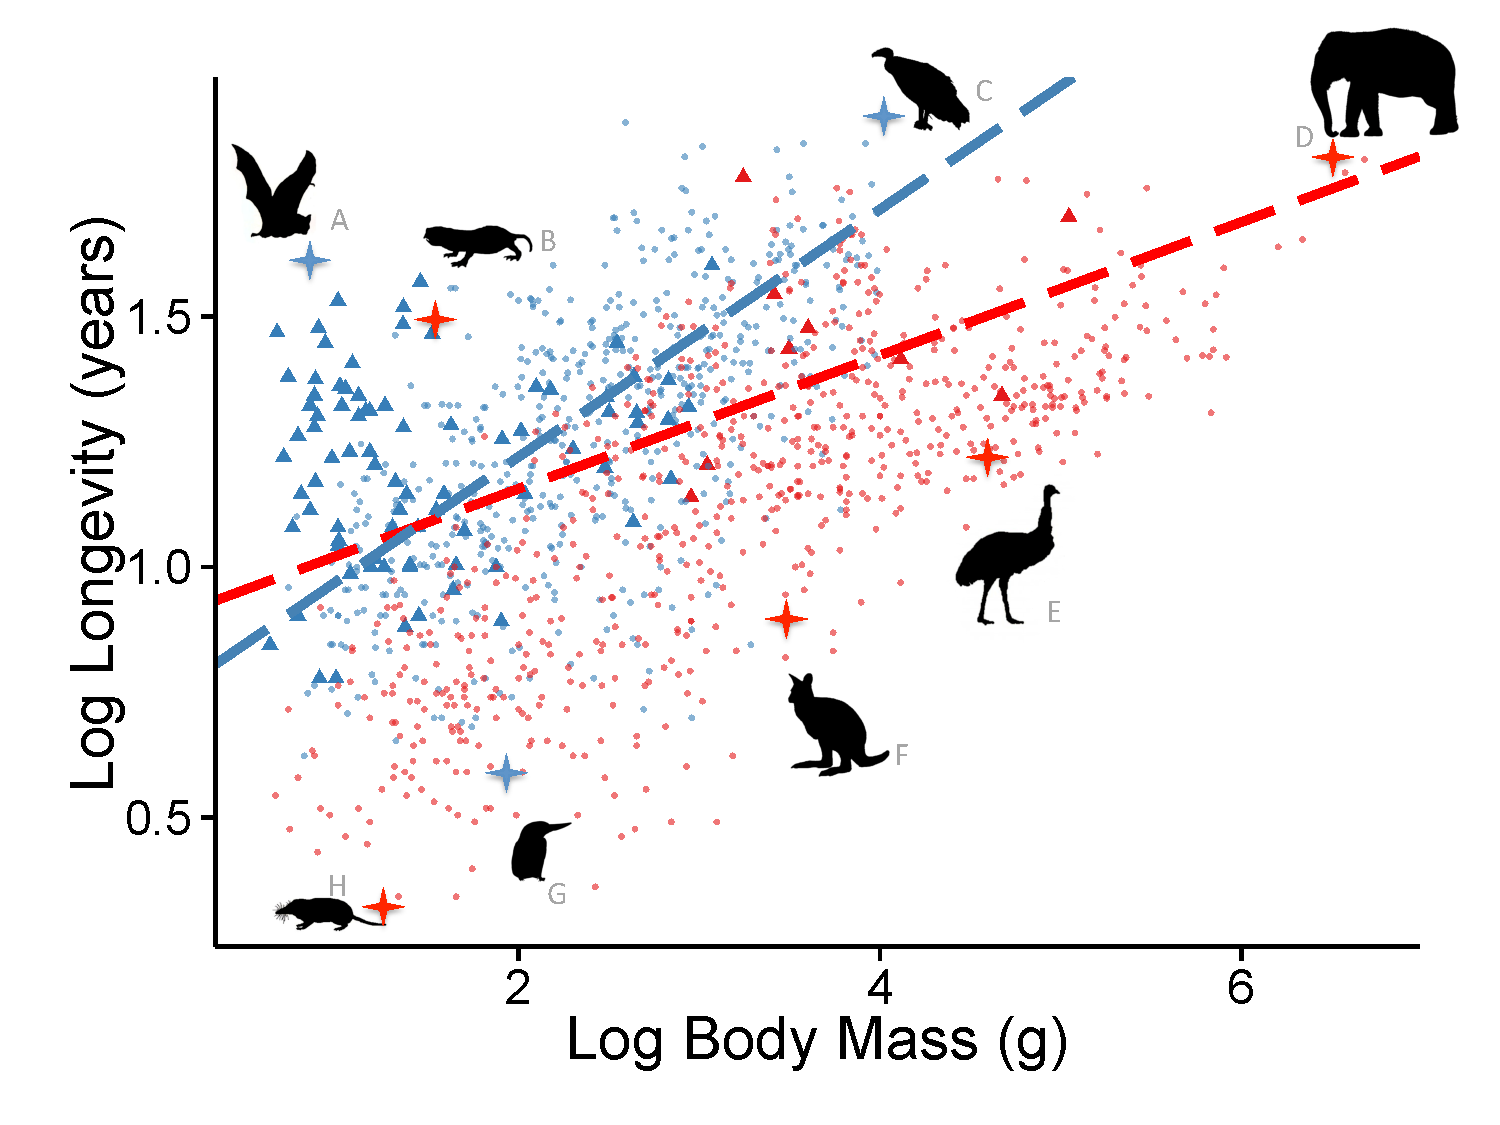
\includegraphics[width=1.0\textwidth]{ch3-longevity/Figure1.pdf}
  \caption[Figure 1.]{Relationships between body mass and maximum lifespan in birds and mammals. Silhouettes highlight a selection of species with much longer or shorter lifespans than expected given their body size. These species are (A) \textit{Myotis brandtii}, Brandt's bat; (B) \textit{Heterocephalus glaber}, Naked mole rat; (C) \textit{Vultur gryphus}, Andean condor; (D) \textit{Loxodonta Africana}, African elephant; (E) \textit{Dromaius novaehollandiae}, Emu; (F) \textit{Dorcopsulus macleayi}, Papuan forest-wallaby; (G) \textit{Ceryle rudis}, Pied kingfisher; and (H) \textit{Myosorex varius}, Forest shrew. Blue points and line represent volant birds and mammals (N = 662; slope = 0.25, intercept = 0.73). Red points and line represent non-volant birds and mammals (N = 706; slope = 0.13, intercept = 0.89). Blue triangles represent bat species and red triangles represent non-volant bird species. Estimates of slopes and intercepts represent back transformed values from mean centred values given in Table 1.}
  \label{figure:Figure 1.}
\end{figure}


The relationships among our ecological variables and lifespan differed between the volant and non-volant subgroups. Within volant taxa, crepuscular species (i.e. those active at dusk and dawn) had significantly shorter lifespans than both diurnal and nocturnal species (Table 2). In contrast, activity period was not associated with lifespan in non-volant species (Table 3). Foraging environment did not influence lifespan significantly in volant species; bats and birds that forage on the ground do not have shorter lifespans than species that forage in the air or in trees (Table 2). Within non-volant species, however, those foraging arboreally have longer lifespans than those foraging terrestrially, and fossorial (i.e. burrowing) species live longer than non-fossorial ones (Table 3).


\begin{table}[h]
  \caption[Table 2.]{Relationship between maximum longevity (years), body mass (g), foraging environment and activity period in 662 volant birds and mammals. Estimates are modal estimates from 500 models. Lower CI = Lower 95\% confidence interval from 500 models. Upper CI = Upper 95\% confidence interval from 500 models. Posterior distribution = distribution of estimates from 500 models.}
  \label{tbl:Table 2.}
  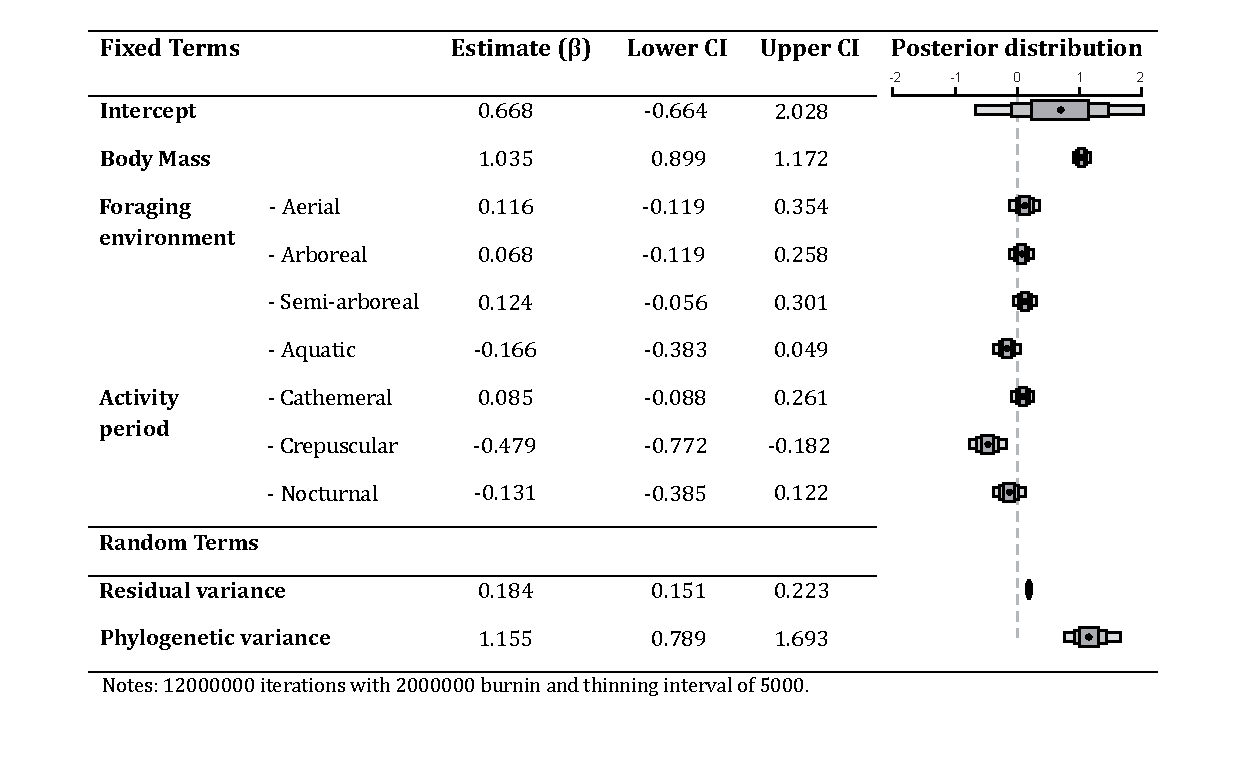
\includegraphics[width=\linewidth]{ch3-longevity/Table2.pdf}
\end{table}


\begin{table}[h]
  \caption[Table 3.]{Relationship between maximum longevity (years), body mass (g), foraging environment, fossoriality and activity period in 706 non-volant birds and mammals. Estimates are modal estimates from 500 models. Lower CI = Lower 95\% confidence interval from 500 models. Upper CI = Upper 95\% confidence interval from 500 models. Posterior distribution = distribution of estimates from 500 models.}
  \label{tbl:Table 3.}
  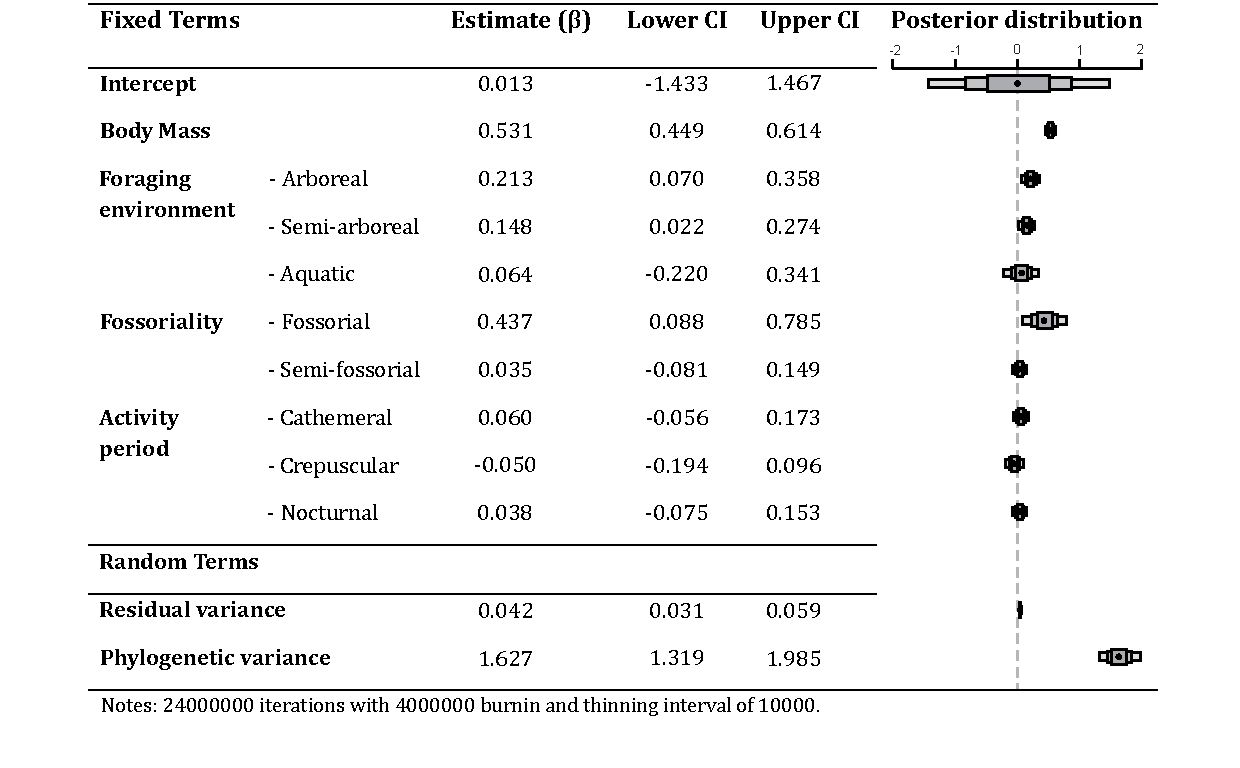
\includegraphics[width=\linewidth]{ch3-longevity/Table3.pdf}
\end{table}


\begin{table}[h!]
  \caption[Table 4.]{Relationship between maximum longevity (months), body mass (g), sociality (eusocial or no-eusocial) and fossoriality (fossorial non-fossorial). Estimates are modal estimates from 25 models. Lower CI = Lower 95\% confidence interval from 25 models. Upper CI = Upper 95\% confidence interval from 25 models. Posterior distribution = distribution of estimates from 25 models.}
  \label{tbl:Table 4.}
  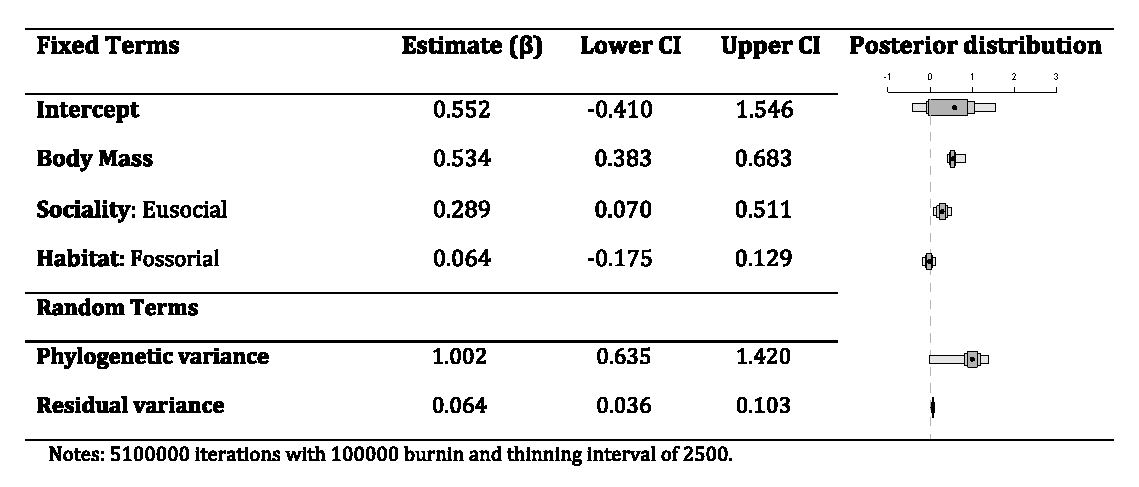
\includegraphics[width=\linewidth]{ch3-longevity/Table4.pdf}
\end{table}



In the supplementary analysis with maximum longevity estimates based on 100 or more records, the models showed qualitatively comparable results to the findings in the main analysis (Appendix 3: Tables A2-A4). When we included BMR as an additional linear covariate into Models 1-3, the results showed similar general trends as those without BMR except with no significant effect of crepuscularity in volant species, no effect of semi-arboreality in non-volant species and a negative correlation between BMR and longevity in non-volant species (Appendix 3: Tables A5-A7).  We also repeated Models 2 and 3 for birds and mammals (rather than volant and non-volant species) separately. The results were qualitatively identical apart from a predictable reduction in the phylogenetic residual term and also a lower combined DIC value for Models 2 and 3 (modal volant and non-volant DIC = 1184) in comparison to a taxonomically split model (modal birds and mammals DIC  = 1227) (Appendix 3: Tables A8-A9). The phylogenetic residual term was high in all of our models (model 1: 1.542; model 2: 1.555; model 3: 1.627; Tables 1-3) but was much lower in the taxonomically split bird and mammal models, as expected given their more restricted phylogenetic scope (birds: 0.371; mammals: 0.936; Appendix 3, Table A10). Finally, the additional analysis of \cite{williams2015ecology} dataset showed that eusociality but not fossoriality (as defined to include both semi-fossorial and fully fossorial species; Table 4).



\section{Discussion}

As predicted, we found that species capable of exploiting high dimensional environments live longer than species of a similar body mass in environments of lower dimensionality. Volant species, in particular those with nocturnal, cathemeral and diurnal activity patterns, lived longer then non-volant species while the longest-lived non-volant species tended to be arboreal or semi-arboreal. The link between these traits and increased lifespan are in line with previous studies on lifespan evolution in endotherms. Among birds, flightless or weakly-flying species (i.e. game birds) have the shortest lifespans \citep{ricklefs2010life,Williams1957,wilkinson2002life} while among mammals, bats live far longer than similarly sized non-volant mammals (ref). Arboreality is also strongly associated with longer lifespans \citep{shattuck2010arboreality} while gliding species, which mix elements of both arboeriality and volancy, also have greater lifespans than expected given their body mass \citep{holmes1994fly}. This increased lifespan is likely associated with the decreased predation pressures associated with living within high dimensional environments.


High dimensional environments may reduce predation risks through providing refuge that predators cannot access and through providing more escape routes in terms of directionality. Prey escape strategies often involve retreating to a refuge that cannot be accessed by the predator in pursuit, such as transiting between terrestrial, arboereal, aquatic or fossorial environments. However these results suggest that this is not a major contributor to lifespan evolution as semi-aquatic and semi-fossorial species show no difference in longevity in comparison to fully terrestrial species. The increased longevity in higher dimensional environments may hence better reflect the increased options available for escape in such habitats. In fact birds species that escape along vertical flight trajectory's (3D) have been found to have longer lifespans in comparison to those that use horizontal escape routes \citep{moller2010up}. 


Another explanation for the disparity between the expected decrease in longevity with due to increased predation rates with body size in high dimensional habitats \citep{pawar2012dimensionality} and these findings is that the environments included within this analysis restrict large predators. Unlike marine environments aerial and arboreal environments several restricts body size through biomechanical constraints. This is seen in the largest known aerial predators, \textit{Argentavis}, reaching only 70 kg \citep{chatterjee2007aerodynamics} while the largest extant terrestrial predators reaching up to 1000 kg \citep{carwardine1995guinness}, with extinct theropods species reaching over 15 tonnes \citep{therrien2007my}. Similarly arboreal predators are restricted by the weight branches can support with the largest such predators, felids, generally restricted to ticker branches. This exclusion of large body size species may also explain the difference in how lifespan scaled with body mass found in volant and non-volant species. While previous studies generated similar slopes for the relationship between log lifespan and log body mass in birds (slope = 0.20) and mammals (slope = 0.22) \citep{lindstedt1981body,hulbert2007life} these analysis show for a given increase in body mass, the lifespans of volant species (modal slope estimate [after converting from mean-centred values] = 0.25) increase significantly more than the lifespans of non-volant species (modal slope estimate [after converting from mean-centred values] = 0.13). This difference in scaling may reflect the relativity predator free existence of large flying species such as found in vultures and albatross.


While habitat dimensionality shows an important effect on longevity, activity patterns in both volant and non-volant species seems to show little association with lifespan. Only crepuscularity in volant species showed an effect with these species having shorter maximum lifespans. This may be a result of crespucuar species being exposed to both diurnal and nocturnal predators resulting in higher extrinsic mortality. For example bat species which emerge earliest are sucesptible to the highest predation levels \citep{jones1994foraging}. The scarcity of crepuscular volant species (N = 16) in our dataset also suggests that specialisation to be active between nocturnal and diurnal periods is a relatively unsuccessful strategy. However, activity period was not related to lifespan in non-volant species, counter to the initial prediction that nocturnal, crepuscular and cathemeral species would be more long-lived, which assumed that diurnal species would be easier for predators to detect. some link. However, there are many additional ways to avoid predation (see below) and many alternative reasons for becoming nocturnal, crepuscular or cathemeral. For example, many large mammals are crepuscular or cathemeral in order to avoid the intense heat of the day in tropical areas, while species such as wolves and hyenas may have become nocturnal to access more prey. Consequently, although nocturnality may decrease extrinsic mortality for some species, it may actually increase it for others.


Within the main analysis fully fossorial species lived longer then similar sized terrestrial species, as expected based on the inferred protection such a lifestyle may provide against predators. However subsequent analysis following \cite{williams2015ecology} showed that this association is more likley to be driven by the levels of eusociality found in fossorial species. Eusociality is also known to increase longevity through the reduce extrinsic mortality in breeding indaviduals. For example eusocial insects, perhaps the most extreme example of such a eusocial system, show a 100-fold increase in lifespan in the colony queens \citep{keller1997extraordinary}. Of the 10 fully fossorial species included in our original analysis the three species which can be best described as eusocial, the naked mole rates \textit{Heterocephalus glaber}; \textit{Cryptomys damarensism}; \textit{Spalax ehrenbergi} have maximum lifespans ranging between 15.5 and 32 years in comparison to the range of 2.5-17 years in the remaining fossorial species. This new analysis suggest that fossoriality itself does not confer additional protection from external mortality. This may be due fossoriality restricting the means of escape once encountered by a predator within the borrow. This result supports the conclusion that dimensionality is a main feature in reducing mortality in the species and may offer a  partial explanation for the exceptional longevity of naked mole rats (Heterocephalus glaber) which live ten times longer than expected, given their body size \citep{buffenstein2002naked}.



 Also following from Peto’s paradox, that cancer incidence does not correlate with body size despite the larger number of cells from which it can potentially develop [40], the increased lifespan afforded through decreased extrinsic mortality in large species can increase selection for molecular controls on senescence related diseases [11]. 


These findings highlight the potential importance of habitat complexity in lifespan evolution. The additional options for escape in such habitats may be a defining feature of throphic interactions within birds and mammals. However the biomechanical limitations associated with volancy and arboerialty, restrict the ability to draw out whether this is the causal factor behind such increased lifespans. Further comparative analysis in marine systems were such body size limitations are less restrictive and were pelagic systems are relatively clear of refuges would provide a further test to the above conclusions. In particular if habitat dimensionality is an important factor in lifespan evolution it would be expected that pelagic species live longer then similar sizes benthic species while accounting for phylogeny. Similarly other groups may help further decouple the effects of fossoriality on life history evolution. In particular comparing the diverse ecologies within reptiles would further test the effects of arboeality and fossoriality on lifespan.

Finally, while the ability to escape some of the main sources of mortality is likely to extend species lifespan and the associations between longevity and volancy, arboerality and eusocialty is clear the direct causal link is still not clear. Theoretical modelling suggests that how mortality is distributed across a species demography is a key determinant in whether that species increases its lifespan. For example reduced extrinsic mortality, especially due to predation, may increase intraspacific competition resulting in what seems as a counter-intuitive reduction in lifespan (current biology paper). To decouple such effects more detailed analysis including mortality rates across species life-histories along with comparative methods which include ecology are needed. By understanding the underpinnings of the evolution of life-history we not only provide an insight into the ecology and evolution of predator-prey interactions provide an important basis on which to view our own and understand our own ageing and  the potential to circumvent it.




\bibliographystyle{PLoS-Biology}
\bibliography{bibfile}




\chapter[Snake]{Ecology and mode-of-life explain lifespan variation in birds and mammals}
\label{chap:Snake}



\begin{figure}[h]
  \centering
  
\includegraphics[width=.30\textwidth]{ch4-snakes/venom.png}
\end{figure}


\begin{quoteshrink}
  ``Always keep your smile. That's how I explain my long life.''
  
\hfill{Jeanne Calment}
\end{quoteshrink}

\begin{abstract}

snakes are great
\end{abstract}

\section{Introduction}

Why are snakes so venamous


\section{Materials and Methods}
\subsection{Data}

Data stuff

\subsection{Analyses}

Models and stuff

\section{Results}


found this

\section{Discussion}

This is what I think
		
\chapter{Conclusion}
\label{chap:conclusions}

So here are my conclusions...

That a nice conclusion.

\section{Future directions}
\label{sec:future-directions}

There's so much more to do!

\subsection{Improving my models}
\label{sec:bett-spec-models}

I'd like to write better analytical models! And try my methods on T rex too.


 


\bibliographystyle{PLoS-Biology}
\bibliography{bibfile}

\formatappendices
\chapter{Supplementary Information to \Chapref{labstudy}}%labstudy is the label for chapter 2.

\section{Additional cool equations}
%basically treat this the same as normal chapters
\label{sec:root-state-calc}
 
This probability is given by the likelihood given that the root is in state
$i$ divided by the sum of the likelihoods over both root states,
$D_{Ri}/(D_{R0}+D_{R1})$.  The overall likelihood is then:
\begin{equation}
  \label{eq:root}
  D_{R} = D_{R0}\frac{D_{R0}}{D_{R0} + D_{R1}} +
  D_{R1}\frac{D_{R1}}{D_{R0} + D_{R1}}
\end{equation}



\end{document}
